\section{Metodología ágil SCRUM}

{Tal y como lo explica la guía de Scrum, es un marco de trabajo, un framework por el cual las personas pueden abordar problemas complejos adaptativos, a la vez que entregan productos del máximo valor posible de forma productiva y creativa, scrum se basa en la teoría de control de procesos empírica o empirismo, que asegura que el conocimiento procede de la experiencia y de tomar decisiones basándose en lo que se conoce.\\

El plan del sprint es creado por todos los miembros del equipo Scrum de forma colaborativa. En esta ceremonia se toman todas las historias de usuario priorizadas y se decide sobre cuáles hacer el Sprint tomando como base el objetivo del sprint y la capacidad del equipo. Se define qué puede entregarse en el Incremento resultante del Sprint que comienza y cómo se conseguirá hacer el trabajo necesario para entregar el Incremento. Si bien Scrum no establece un método para estimar es recomendable utilizar alguno como, por ejemplo, la estimación en puntos de historia para cada uno de los elementos del sprint backlog.

	\subsection{Personas y roles del Proyecto}
	{\begin{figure}[H]
		\centering
		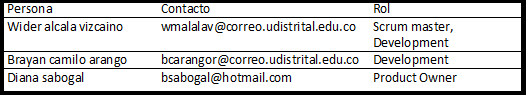
\includegraphics[width=1\linewidth]{development/roles.png}
		\caption{Roles y actores}
	\end{figure}}
	\begin{center}
		\textbf{Fuente:} Propia.
	\end{center}
	\hfill

	\subsection{Pila del Sprint}
	{En esta sección se describe de forma detallada los requisitos o tareas que va a desarrollar el equipo de trabajo en cada iteración.
	
		\subsubsection{Responsabilidades del gestor de producto}
		{Presencia en las reuniones en las que el equipo elabora la pila del sprint. Resolución de dudas sobre las historias de usuario que se descomponen en la pila del sprint}
		
		\subsubsection{Responsabilidades del equipo técnico}
			\begin{itemize}
				\item Elaboración de la pila del sprint.
				\item Resolución de dudas o comunicación de sugerencias sobre las historias de usuario con el gestor del producto.
			\end{itemize}
	}

	\subsection{Pila del Producto}
	{A continuación, se define la lista de requisitos o requerimientos funcionales que debe cumplir el sistema de acuerdo a la solicitud del cliente.
		
	El requisito principal del proyecto es crear un prototipo que permita la gestión de micro transacciones entre sus usuarios.\\
		
		\begin{itemize}
			\item \textbf{Modulo administrador:} permite la gestión de usuarios administrando los permisos, menús etc. según cada uno de los perfiles asignados.
			\item \textbf{Registrar préstamo:} Permitir el registro del préstamo de una forma intuitiva.
			\item \textbf{Obtener préstamo:} Permitir a través de un código QR, asignarse un préstamo.
			\item \textbf{Pagar préstamo y aceptar pagos:} Movimientos realizados al préstamo.
		\end{itemize}
	
	}

	\subsection{Primera Iteración}
	{La primera fase del proyecto será desarrollar las actividades referentes a la parte administrativa donde se van a gestionar los permisos, perfiles y menús del prototipo.\\
	
	\begin{figure}[H]
			\centering
			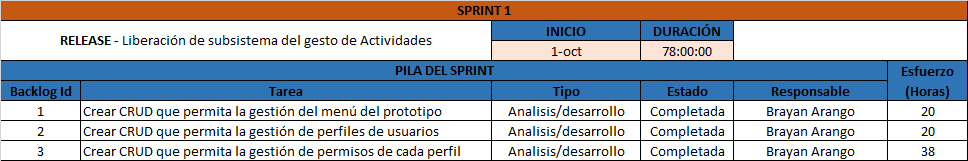
\includegraphics[width=1\linewidth]{development/sprint1.png}
			\caption{Sprint 1}
	\end{figure}
	\begin{center}
		\textbf{Fuente:} Propia.
	\end{center}

	\begin{itemize}
		
		\item \textbf{Incremento:} Luego de asignar las tareas relacionadas con el módulo de administración de usuarios del proyecto se obtiene el primer incremento, el cual consiste de todos los CRUD con los cuales es posible otorgar permisos a los usuarios y perfiles.
			
		
		\item Listar menús
			\begin{figure}[H]
				\centering
				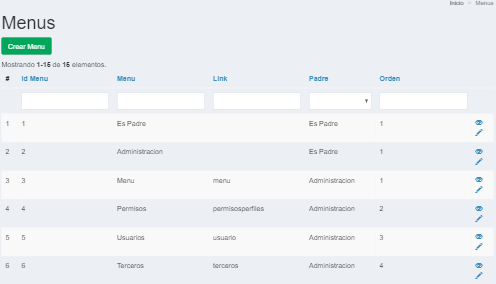
\includegraphics[width=1\linewidth]{development/listarmenu.png}
				\caption{Lista de menus - Tru\$tMe}
			\end{figure}
			\begin{center}
				\textbf{Fuente:} Propia.
			\end{center}
			\hfill \break
		
		\item Crear menús
		\begin{figure}[H]
			\centering
			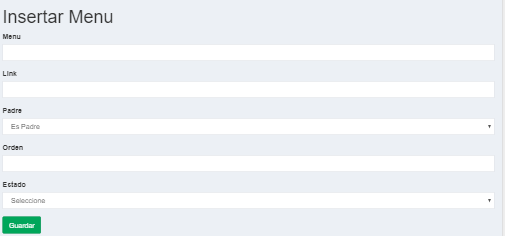
\includegraphics[width=1\linewidth]{development/crearmenu.png}
			\caption{Creación de menus - Tru\$tMe}
		\end{figure}
		\begin{center}
			\textbf{Fuente:} Propia.
		\end{center}
	
		\item Actualizar menú
		\begin{figure}[H]
			\centering
			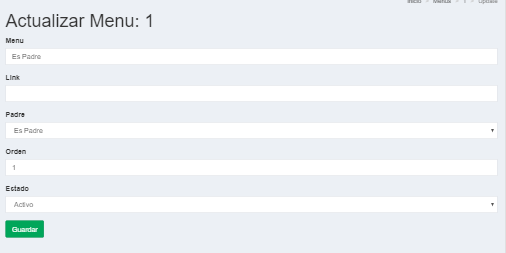
\includegraphics[width=1\linewidth]{development/actualizarmenu.png}
			\caption{Actualización de menus - Tru\$tMe}
		\end{figure}
		\begin{center}
			\textbf{Fuente:} Propia.
		\end{center}
		
		\item Listar perfiles
		\begin{figure}[H]
			\centering
			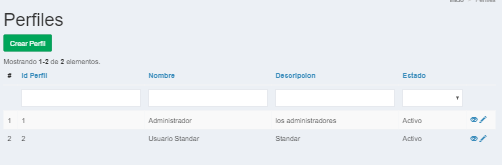
\includegraphics[width=1\linewidth]{development/listarperfiles.png}
			\caption{Listar perfiles - Tru\$tMe}
		\end{figure}
		\begin{center}
			\textbf{Fuente:} Propia.
		\end{center}
		\hfill
		
		\item Crear perfiles
		\begin{figure}[H]
			\centering
			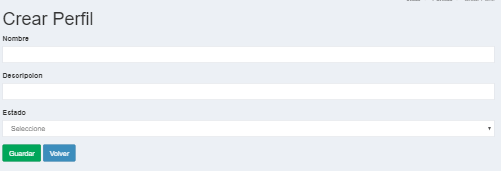
\includegraphics[width=1\linewidth]{development/crearperfiles.png}
			\caption{Creación de perfiles - Tru\$tMe}
		\end{figure}
		\begin{center}
			\textbf{Fuente:} Propia.
		\end{center}
		\hfill \break
		\hfill \break
		\hfill \break
		
		\item Actualizar perfiles
		\begin{figure}[H]
			\centering
			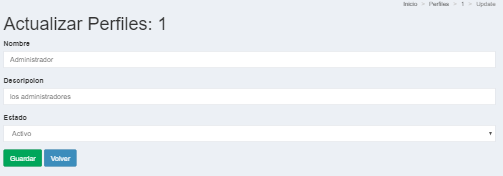
\includegraphics[width=1\linewidth]{development/actualizarperfiles.png}
			\caption{Actualización de perfiles - Tru\$tMe}
		\end{figure}
		\begin{center}
			\textbf{Fuente:} Propia.
		\end{center}
	
		\item Otorgar permisos a un perfil
		\begin{figure}[H]
			\centering
			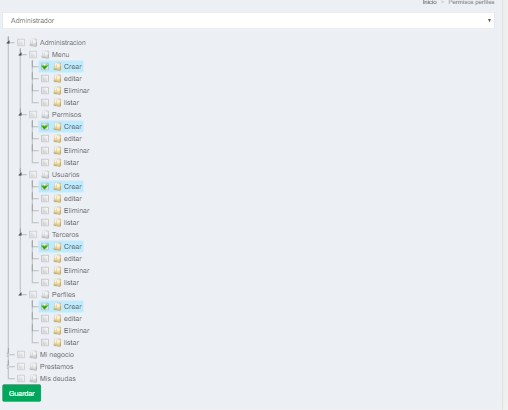
\includegraphics[width=1\linewidth]{development/otorgarpermisos.png}
			\caption{Otorgació de permisos - Tru\$tMe}
		\end{figure}
		\begin{center}
			\textbf{Fuente:} Propia.
		\end{center}
		
		 
	\end{itemize}
		

		
	}

		\subsection{Segunda Iteración}
		{La segunda fase del proyecto será desarrollar las actividades referentes a la creación del CRUD referente a la creación del préstamo.\\
			
			\begin{figure}[H]
				\centering
				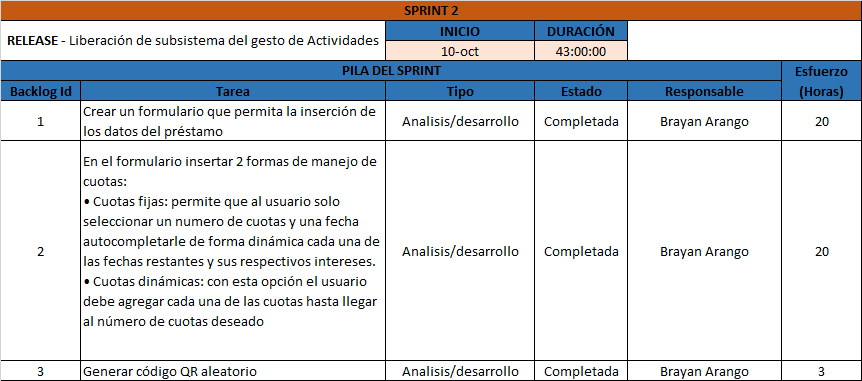
\includegraphics[width=1\linewidth]{development/sprint2.png}
				\caption{Sprint 2}
			\end{figure}
			\begin{center}
				\textbf{Fuente:} Propia.
			\end{center}
			
			\begin{itemize}
				
				\item \textbf{Incremento:} Luego de asignar las tareas relacionadas con el módulo de guardar préstamo se obtiene el segundo incremento, el cual consiste en el formulario de crear préstamo.
				
				
				\item Guardar préstamos
				\begin{figure}[H]
					\centering
					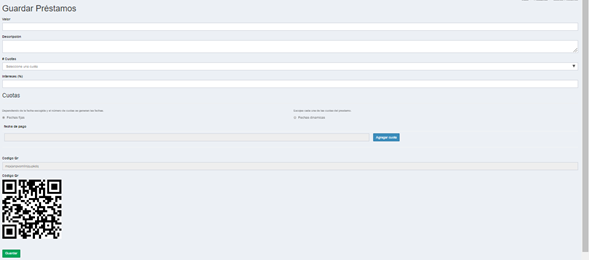
\includegraphics[width=1\linewidth]{development/guardarprestamos.png}
					\caption{Guardar préstamos - Tru\$tMe}
				\end{figure}
				\begin{center}
					\textbf{Fuente:} Propia.
				\end{center}		
					
			\end{itemize}
			
			
			
		}

		\subsection{Tercera Iteración}
		{La tercera fase del proyecto será desarrollar las actividades referentes a la obtención de los préstamos.\\
			
			\begin{figure}[H]
				\centering
				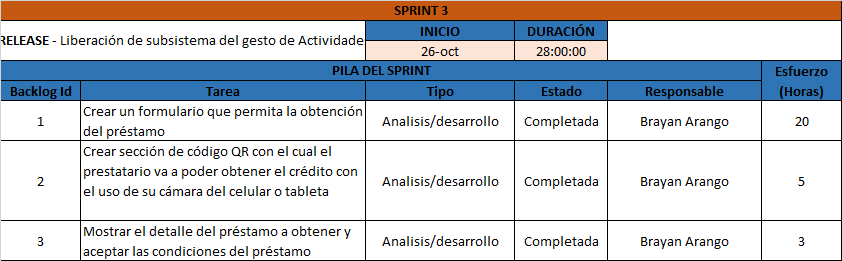
\includegraphics[width=1\linewidth]{development/sprint3.png}
				\caption{Sprint 3}
			\end{figure}
			\begin{center}
				\textbf{Fuente:} Propia.
			\end{center}
				
			\begin{itemize}
				
				\item \textbf{Incremento:} Luego de asignar las tareas relacionadas con el módulo de obtener préstamo se obtiene el tercer incremento, el cual consiste en el formulario para que el prestatario pueda adquirir un préstamo.
				
				
				\item Escanear QR
				\begin{figure}[H]
					\centering
					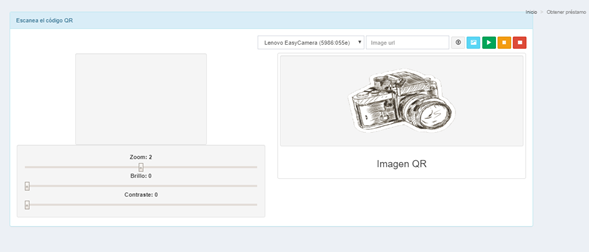
\includegraphics[width=1\linewidth]{development/escanearqr.png}
					\caption{Escanear QR - Tru\$tMe}
				\end{figure}
				\begin{center}
					\textbf{Fuente:} Propia.
				\end{center}
					
				\item Resumen de préstamos
				\begin{figure}[H]
					\centering
					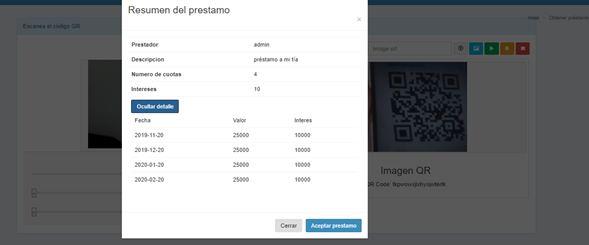
\includegraphics[width=1\linewidth]{development/resumenprestamos.png}
					\caption{Resumen de préstamos - Tru\$tMe}
				\end{figure}
				\begin{center}
					\textbf{Fuente:} Propia.
				\end{center}
	
				
			\end{itemize}
			
			
			
		}

}
	


